\documentclass[12pt, amsmath]{revtex4-2}
\usepackage{hyperref} %Make references into hyperlinks.
\usepackage{subfig}
\usepackage{mathrsfs} % for \mathscr -> scri
\usepackage{xfp} % for fpeval -> floating point expression
\usepackage{graphicx}
\usepackage{amsmath}
\usepackage{cleveref}
\usepackage{xcolor}

\usepackage{ulem} %for \sout

\usepackage{float}
\input{CQGformat.input}


\newcommand\lam{\lambda}
\newcommand\EN{\mathcal{E}}
\newcommand\ANG{\mathcal{L}}
\DeclareMathOperator{\arctanh}{arctanh}
\DeclareMathOperator{\sn}{\mathsf{sn}}
\DeclareMathOperator{\cn}{cn}
\DeclareMathOperator{\dn}{dn}
\DeclareMathOperator{\am}{\mathsf{am}}
\DeclareMathOperator{\amz}{\xi_z}
\DeclareMathOperator{\snr}{sin(\xi_r)}
\DeclareMathOperator{\cnr}{cos(\xi_r)}
\DeclareMathOperator{\amr}{\xi_r}

\newcommand{\elK}{\operatorname{\mathsf{K}}}%use this%
\newcommand{\elE}{\operatorname{\mathsf{E}}}%use this%
\newcommand{\elF}{\operatorname{\mathsf{F}}}%use this%
\newcommand{\elPi}{\operatorname{\mathsf{\Pi}}}%use this%

\newcommand{\mvdm}[1]{{\color{orange}{#1}}}
\newcommand{\cd}[1]{{\color{blue}{#1}}}

\begin{document}
\title{Kerr-fully Diving into the Abyss: Analytic Solutions to Plunging Geodesics in Kerr}
\author{Conor Dyson$^1$,  Maarten van de Meent$^{1,2}$}

\address{$^1$ Niels Bohr International Academy, Niels Bohr Institute, Blegdamsvej 17, 2100 Copenhagen, Denmark}
\address{$^2$ Max Plank Institute for Gravitational Physics (Albert Einstein Institute), Potsdam-Golm, Germany}



\begin{abstract}

We present closed-form solutions for plunging geodesics in the extended Kerr spacetime using Boyer-Lindquist coordinates. Our solutions directly solve for the intricate dynamics of generic timelike plunges, we also specialise to the case of test particles plunging from a precessing innermost stable circular orbit (ISSO). We find these solutions in the form of elementary and Jacobi elliptic functions parameterized by Mino time. In particular, we demonstrate that solutions for the ISSO case can be determined almost entirely in terms of elementary functions, depending only on the spin parameter of the black hole and the radius of the ISSO. This extends recent work on the case of equatorial plunges from the innermost stable circular orbit \cite{Mummery:2022ana}. Furthermore, we introduce a new equation that characterizes the radial inflow from the ISSO to the horizon, taking into account the inclination. For ease of application, our results have been incorporated in the {\tt KerrGeodesics} package in the Black Hole Perturbation Toolkit \cite{BHPToolkit}.

\end{abstract}
\section{Introduction}

Analysing the geodesic structure of a spacetime is one of the foundational means of understanding it in its unperturbed state. The geodesics of the Kerr spacetime have been extensively studied since its original derivation \cite{Kerr:1963ud}. A critical step in the calculation of the geodesics in Kerr was the discovery of a fourth constant of motion, the Carter constant $Q$ \cite{Carter:1968rr}, which along with the normalisation of the Lagrangian, the conserved energy $\EN$ and the angular momentum $\ANG$ allow for the full integrability of the geodesic equations of motion. While exact solutions for various special cases had been derived (e.g, see~\cite{Chandrasekhar:579245} or \cite{Wilkins:1972rs}) no real effort was made to tackle the generic case until the start of the 21st century. Without getting explicit solutions for the geodesics themselves, \cite{Schmidt:2002qk}~found exact expressions for the orbital frequencies w.r.t. coordinate time of generic bound orbits. The introduction of the Mino time parameterisation \cite{Mino:2003yg} subsequently allowed for the full decoupling of the problem in an much simpler manner to previous approaches~\cite{Carter:1968rr}.
This opened the door for finding analytic solutions to generic bound geodesics in Kerr~\cite{Fujita:2009bp} as a system of piecewise smooth functions, which were then notably simplified through analytic continuation~\cite{vandeMeent:2019cam}.

The full class of analytic solutions to  Kerr-de Sitter and Kerr-anti-de Sitter space-times has been found in \cite{Hackmann:2010zz} their generic form, presented in the form of Weierstrass elliptic and hyperelliptic Kleinian functions, which can make them cumbersome to deal with. This work also provided part of the motivation for deriving a more explicit solution for null geodesics in the exterior of Kerr in terms of Jacobi elliptic functions \cite{Gralla:2019ceu}. Recent work has subsequently derived these equations for the specified case of bound null geodesics \cite{Omwoyo2022:2212.10492v1}, relevant in pursuit of forming tight constraints on Black Hole parameters by observations of the photon ring using the Event Horizon Telescope \cite{broderick2022photon}.

Recently Mummery and Balbus \cite{Mummery:2022ana} have  derived a much simplified analytic solution for the equatorial case of plunging timelike geodesics which asymptote from the innermost stable circular orbit (ISCO). In this work, they also provide a simple expression for the equatorial radial inflow from the ISCO relevant to the study of accretion disk dynamics. In practice, these systems won't always be confined to the equatorial plane, motivating generalising of this result to the inclined (i.e. non-spin aligned or precessing) case, as we will do in this paper.

The work presented here is further motivated by the fundamental role that geodesics play in the gravitational self-force approach to solving the relativistic dynamics of binary black holes \cite{Barack:2018yvs}. In this approach the  dynamics are expanded in powers of the mass-ratio between to two black holes. In this scheme, the zeroth approximation to the motion of the lighter secondary component is given by a geodesic in the Kerr geometry generated by the (heavier) primary black hole. At higher orders, this motion is corrected by an effective force term, the gravitational self-force, causing the system to evolve.
During the inspiral phase this evolution can be solved using a 2-timescale formalism\cite{Hinderer:2008dm,
Pound:2021qin, Miller:2020bft}, adiabatically evolving the system along a sequence of bound geodesics. The 2-timescale formalism breaks down as the system approaches the last stable orbit around the black hole, where it enters a transition regime governed by a new intermediate timescale \cite{Buonanno:2000ef, Ori:2000zn, OShaughnessy:2002tbu, Sperhake:2007gu} connecting the dynamics to a geodesic plunging into the primary black hole.

Development of the gravitational self-force formalism was originally motivated by the need for producing accurate gravitational waveforms for the observation of extreme mass-ratio inspirals (EMRIs) with the planned space-based gravitational wave observatory LISA. EMRIs are expected to have mass-ratios of order $10^{-5}$, and will therefore spend hundreds of thousands of orbits in the strong field regime of the inspiral phase. Consequently, the handful of orbits represented by the transition and plunge phases are generally expected to provide a negligible contribution to the total signal. However, over time evidence has mounted
\cite{LeTiec:2011bk,Sperhake:2011ik,LeTiec:2011dp,Nagar:2013sga,LeTiec:2013uey,LeTiec:2017ebm,vandeMeent:2016hel,vandeMeent:2020xgc,Wardell:2021fyy,Ramos-Buades:2022lgf} suggesting that the self-force formalism can produce accurate results at much higher mass-ratios, and possibly even for comparable mass binaries. This has inspired further investigations of both the transition regime \cite{Compere:2021zfj,   Apte:2019txp,Burke:2019yek, Compere:2019cqe, Compere:2021iwh, Compere:2021zfj} and the gravitational waves produced during the plunge and the resulting ringdown \cite{Folacci:2018cic, Hughes:2019zmt, Lim:2019xrb}. In this work we support the latter by providing generic closed-form analytic solutions for plunging geodesics.

The plan of this paper is as follows, in section \ref{sec:GeodesicEquations} we begin with an introduction on the geodesics equations of Kerr and provide explicit definitions for the related conserved quantities. In section \ref{sec:ISSO} we then focus our attention on the special case of plunging timelike geodesics which asymptote from the inner most stable precessing circular orbit (ISSO). From these equations we determine the exact and two approximate expressions for the rate of radial inflow from the ISSO to the horizon, with a corresponding error analysis allowing one to choose the equation that is suitable for their purposes. We then go on to determine the fully analytic solutions to these geodesic equations for ISSO plunges. In the case of ISSO plunges we find that we can fully parameterised the solutions by a black hole spin $(a)$ and a chosen value of ISSO radius $(R_I)$. The value of $R_I$ we choose uniquely determines the maximum inclination of the precessing circular orbit to which the geodesic aymptotes, either in prograde or retrograde. The choice of $R_I$ is limited to a range of allowed values for a given $(a)$ which can be found in~\ref{app:ISSOrange}. Finally in section \ref{sec:deeplybound} of this work we then go on to determine the novel fully analytic expressions for generic timelike plunging geodesics in the Kerr spacetime. We work in geometric units where G = c = 1.


\section{Geodesic Equations}\label{sec:GeodesicEquations}
We work in modified Boyer-Lindquist coordinates $(z = cos(\theta))$ with $M =1$ and $a$ given as the spin of the black hole. Defining $\Sigma =(r^2+a^2z^2)$ , $\Delta = (r-r_{+})(r-r_{-})$ with 
\begin{align}
    r_{\pm} &:= 1 \pm \sqrt{1-a^2}
\end{align}
the inner and outer event horizons. The symmetries of the Kerr geometry provide two constants of motion,
\begin{align}
    \EN &:= -u^{\nu}g_{\mu\nu}\left(\frac{\partial}{\partial t}\right)^{\nu} \text{and}\\
    \ANG &:=  u^{\nu}g_{\mu\nu}\left(\frac{\partial}{\partial \phi}\right)^{\nu} 
\end{align}
 the conserved energy and angular momentum respectively, and where $ g_{\mu\nu}$ is the Kerr metric tensor in modified Boyer-Lindquist coordinates. The third constant of motion $Q$ is the Carter constant \cite{Carter:1968rr} which arises in some spacetimes exhibiting Type D symmetry \cite{Walker:1970un}, which includes the Kerr family of solutions. It arises as a result of a killing tensor given by $\nabla_{(a}\mathcal{K}_{bc)} = 0$. In Kerr this killing tensor is found to be  
\begin{align}
    \mathcal{K}_{\mu\nu} &:= 2\Sigma l_{(\mu} n_{\nu)} + r^2 g_{\mu\nu}
\end{align}
Where $l_{\mu}$ and $n_{\nu}$ are the principal null vectors of the Kinnersly tetrad \cite{Kinnersley:1969zza} defined by $l^{\mu} = [\frac{r^2+a^2}{\Delta}, 1 , 0, \frac{a}{\Delta} ]$ and $n^{\nu} = \frac{1}{ 2\Sigma}[r^2+a^2, -\Delta , 0, a ] $. The Carter constant is then given by 
\begin{align}
    Q:= u^{\mu}\mathcal{K}_{\mu\nu}u^{\nu} - (\ANG-a\EN)^2.
\end{align}

Taking the normalisation of the 4-velocity to be the final constant of motion and setting it to -1 for timelike geodesics the equations for geodesic motion in Kerr are subsequently given by \cite{Carter:1968rr}
\begin{align}
    &\begin{aligned}\label{eq:radialeom}
        \left(\frac{dr}{d\lambda}\right)^2 
        &= (\mathcal{E}(r^2+a^2)-a\mathcal{L})^2-\Delta(r^2+(a\mathcal{E}-\mathcal{L})^2+Q)\\
        &= (1-\EN^2)(r_1-r)(r_2-r)(r_3-r)(r-r_4) \\
        &= R(r), 
    \end{aligned}\\
    &\begin{aligned}\label{eq:polareom}
        \left(\frac{dz}{d\lambda}\right)^2 &= Q-z^2(a^2(1-\EN^2)(1-z^2) + \mathcal{L}^2+Q)\\
        &= (z^2-z_1^2)(a^2(1-\EN^2) z^2-z_2^2)\\
        &= Z(z),
    \end{aligned}\\
    &\;\;\begin{aligned}\label{eq:timeeom}
        \frac{dt}{d\lambda} &= \frac{(r^2+a^2)}{\Delta}(\mathcal{E}(r^2+a^2)-a\mathcal{L})-a^2\mathcal{E}(1-z^2)+a\mathcal{L},\;\;\; \text{and}
    \end{aligned}\\
    &\;\;\begin{aligned}\label{eq:azimuthaleom}
        \frac{d\phi}{d\lambda} &= \frac{a}{\Delta}(\mathcal{E}(r^2+a^2)-a\mathcal{L})+\frac{\mathcal{L}}{1-z^2}-a\mathcal{E},
    \end{aligned}
\end{align}
where we have specialised to working in Mino(-Carter) \cite{Mino:2003yg} time given by 
\begin{equation}
    d\tau = \Sigma d\lam.
\end{equation}
By taking advantage of the Mino time parameterisation we see that the equations of motion fully decouple and can be solved hierarchically. This is done by first solving for $r(\lam)$ and $z(\lam)$ and then naturally solving the equations in the form $t(r,z,\lam) = t_r(r)+t_{z}(z) - a \EN \lam$ and $\phi(r,z,\lam) = \phi_r(r)+\phi_{z}(z) + a\ANG\lam $, at this point the solutions for $r(\lam)$ and $z(\lam)$ can be directly subbed in to attain $t(\lam)$ and $\phi(\lam)$. Writing the radial equation in its explicit form Eq.~\eqref{eq:radialeom} also makes clear that the  distinction between bound and plunging orbits is fully determined by the root structure of our fourth order polynomial $R(r)$. In particular we see that plunges occur when we have bound motion between some roots $r_i,r_j$ of $R(r)$ with $r_i<r_{-} < r_{+} < r_j$. In this work, we restrict to geodesics with $\EN<1$, which implies that the radial potential $R(r)$ is negative in the limit $r\to\infty$, ensuring that the geodesic is bound to the Kerr black hole. Moreover, since $R(r_{\pm})>0$ it guarantees that there is at least one real root of $R(r)$ outside $r_+$. A less obvious implication comes from the polar equation~\eqref{eq:polareom}. Rewriting the polar potential as
\begin{equation}
    Z(z) = (1-z^2)Q-z^2(a^2(1-\EN^2)(1-z^2) + \mathcal{L}^2),
\end{equation}
it becomes apparent that when $\EN<1$ the polar equation has solutions with $-1<z<1$ if and only if $Q\geq 0$. For the radial potential this implies that $R(0)\leq 0$, and consequently that there exist at least one real root of the radial equation between $r=0$ and the inner horizon. We thus find that for any values of $\EN<1$ and $Q\geq 0$, there exists a plunging geodesic. It is important to note that the case of $\EN>1$ with $Q<0$ contributes to a small subset of aloud parameter space for which a real solution actually exists however its dynamics are quite interesting as by a brief analysis of the equations of motion one can see that what this would give a test particle which plunges from infinity and poloidally oscillating around some $z_0 \neq 0$.


Generically, a plunging geodesic will eternally oscillate between two turning points of the radial potential and return to the same radial point after a finite amount of Mino (and proper) time. Geometrically, this corresponds to geodesic diving into the Kerr black hole passing through the two horizons before being scattered back out, passing the horizons in reversed order and exiting in a different asymptotically flat region of the maximally extended Kerr solution, as shown in the Penrose diagram in Fig.~\ref{fig:penrose}.

\begin{figure}[tb!]
    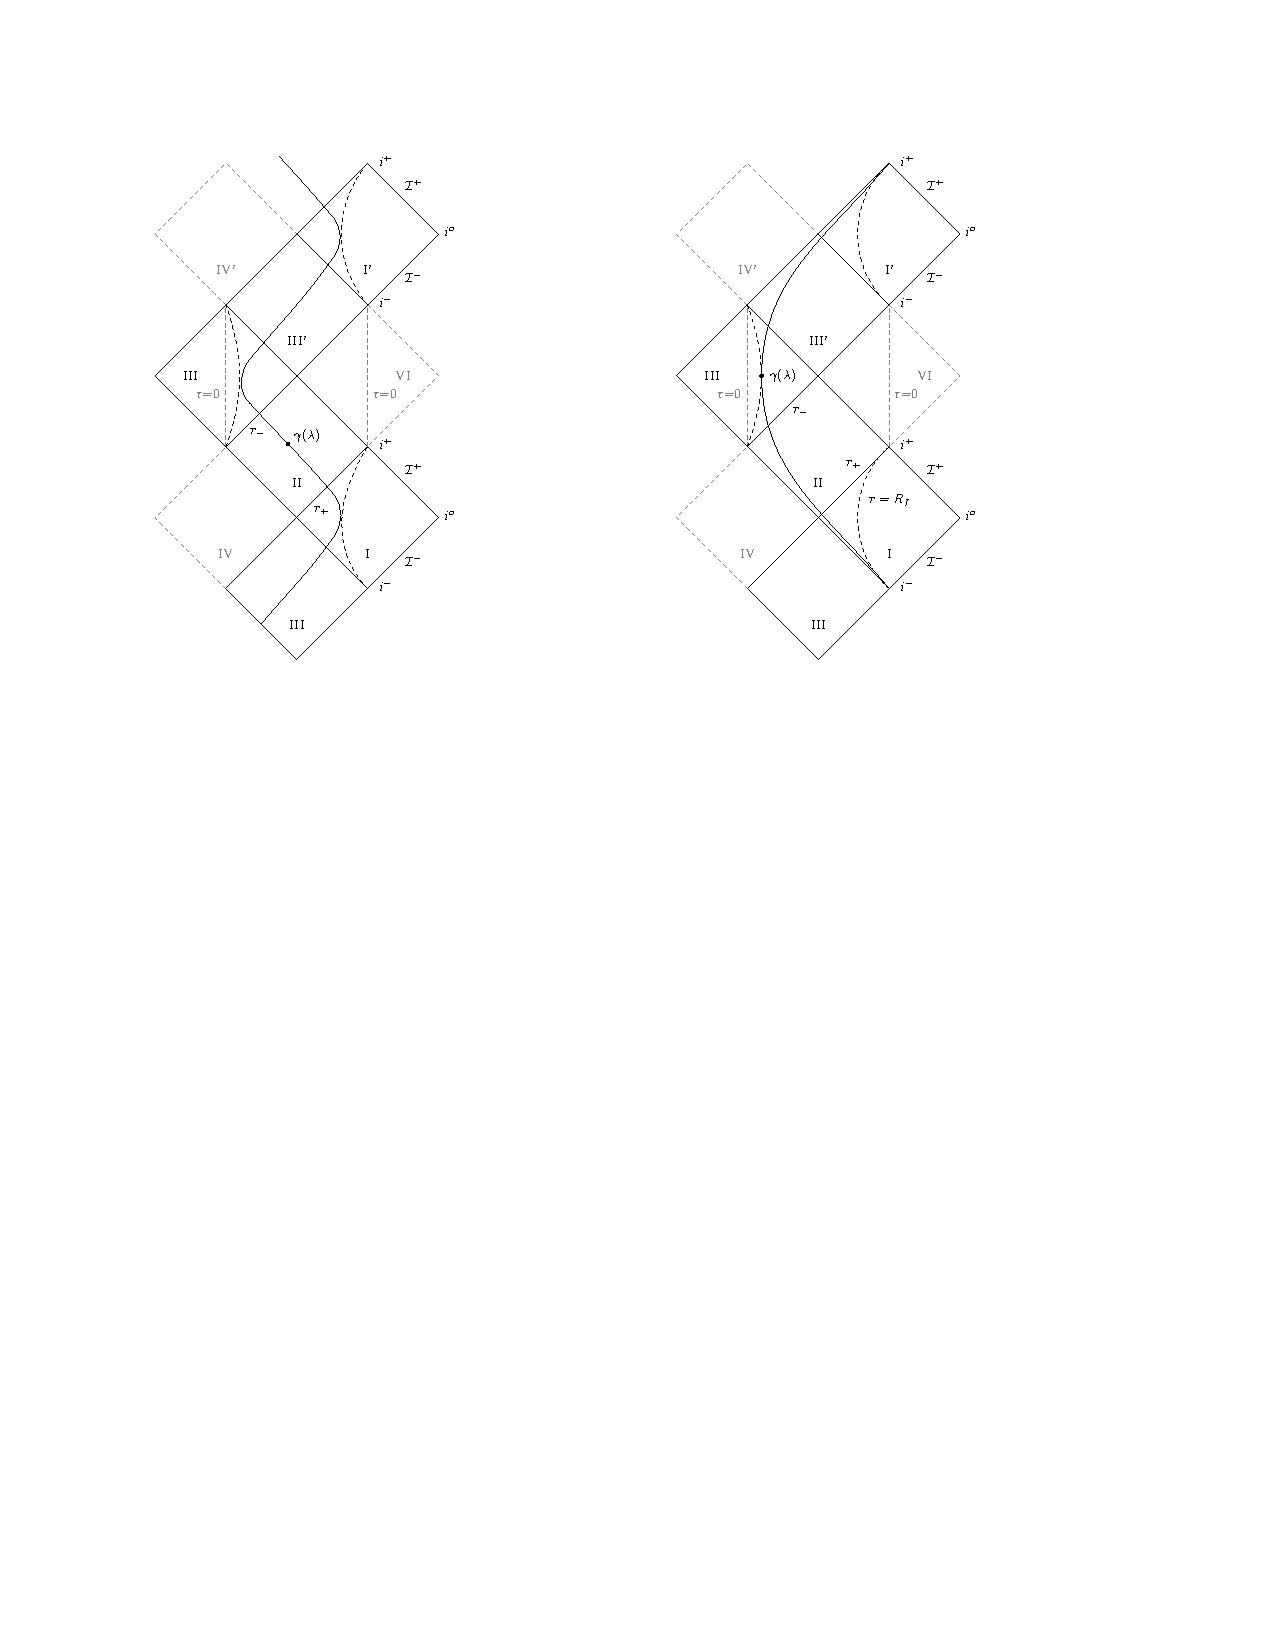
\includegraphics[width=130mm]{PenrosePlot.pdf}
        %\input{tiks-penrose.input} 
    \caption{Left Image: Penrose diagram of a generic plunge orbit where by the solutions oscillate between the largest root of $R(r)$ which is less than $r_-$ and the smallest roots of $R(r)$ greater than $r_+$. Right Image: Penrose diagram of plunge which asymptote to $r_I$ as $\lam\rightarrow \pm\infty$ here $\gamma(\lam)$ represents the geodesic in question. }
     \label{fig:penrose}
\end{figure}
Exceptions to this picture occur for equatorial trajectories and when one of the bounding roots has a multiplicity greater than one. In the first case $Q=0$, which  implies that $r=0$ is a root of the radial equation. If this is the inner turning point of the geodesic, the plunge will start and end on the singularity after a finite amount of Mino (and proper) time. In the second case, approaching the the root with higher multiplicity takes an infinite amount of Mino (and proper) time. In Section~\ref{sec:ISSO}, we will see the physically relevant case where the outer turning point of the solution is a triple root, i.e. lies on the  innermost precessing stable circular orbit (ISSO), where the radial solution takes a particularly simple form generalizing the result of~\cite{Mummery:2022ana}. The right panel in Fig.~\ref{fig:penrose} shows this edge case trajectory in a Penrose diagram.


In the generic case, we know at least two of the four roots of $R(r)$ are real. The other two roots are either both real or both complex. If the other two roots are real they come in a pair that lies either entirely outside the outer turning point, entirely between the inner turning point and $r=0$, or entirely in the $r<0$ region. In the first of these cases, the plunging orbit exists inside of a normal bound orbit, a case sometimes referred to as  a ``deeply bound'' orbit. The solutions for cases with 4 real roots turn-out to be a straightforward generalization from the solutions of~\cite{Fujita:2009bp,vandeMeent:2019cam}. The derivation of the complex case will turn out to be substantially more involved.


\section{The Innermost Precessing Stable Circular Orbit}\label{sec:ISSO}

We begin by determining the solutions for plunges which asymptote to the innermost precessing stable circular orbit (ISSO). In this case the radial potential $R(r)$ is imbued with a triple root at the ISSO radius $r=r_I$. Two of these roots come from the fact that the ISSO must be a stable precessing circular orbit and the additional root at this point arises from the fact we are looking specifically at the innermost of these orbits meaning $R(r)$ must also inflect at this point. As a result we determine a radial equation of the form 
\begin{align}\label{eq:ISSOradialeom}
        \left(\frac{dr}{d\lambda}\right)^2 
        &=(1-\EN^2)(r_I-r)^3(r-r_4)
\end{align}
By equating Eq.~\eqref{eq:radialeom} with Eq.~\eqref{eq:ISSOradialeom} we find that you immediately obtain the result,
\begin{equation}
    r_4 = \frac{a^2Q}{(1-\EN^2)r_{I}^{3}},
\end{equation}
from equating the coefficients of the fourth order in $r$ term. We also find the roots of the polar equation to be given by \cite{Gralla:2019ceu},
\begin{subequations}\label{Equations of Motion}
    \begin{align}
        z_1 &= \sqrt{\frac{1}{2}\left(1+\frac{\mathcal{L}^2+Q}{a^2(1-\EN^2)}-\sqrt{\left(1 + \frac{\mathcal{L}^2+Q}{a^2(1-\EN^2)}\right)^2-\frac{4Q}{a^2(1-\EN^2)}}\right)},\\
         z_2&=\sqrt{ \frac{a^2(1-\EN^2)}{2}\left(1+\frac{\mathcal{L}^2+Q}{a^2(1-\EN^2)}+\sqrt{\left(1 + \frac{\mathcal{L}^2+Q}{a^2(1-\EN^2)}\right)^2-\frac{4Q}{a^2(1-\EN^2)}}\right)}.
    \end{align}
\end{subequations}
Finally, we define
\begin{equation}\label{Equations of Motion}
        k_z = a\sqrt{(1-\EN^2)}\frac{z_1}{z_2},
\end{equation}
as a quantity which will recurrently show up throughout this work.

\subsection{Determining the Conserved quantities}

At this point it is important to note that in order to enforce our geodesics asymptote to the ISSO we have restricted ourselves to two degrees of freedom. Naturally these two degrees of freedom can be set by picking a black hole spin ($a$) and maximum orbital angle of inclination $\theta_{max} \in (-\frac{\pi}{2},\frac{\pi}{2})$. This then determines a unique $r_I$. The more astrophysically interesting case however is when we invert this relation to set our parameterisation in terms of $(a,r_I)$. Doing this we then find that for each value of $a$ there exists a range of allowed $r_I$'s each of which corresponds to a unique inclination either in prograde or retrograde. Parameterisation by $r_{I}$ is astrophysically favorable as a model dependent observable to detectors such as the Event Horizon Telescope \cite{2019ApJS..243...26P}. We also provide analytic solutions to the allowed ranges of $r_I$ denoted $R_{I, \rm max}$ and $R_{I, \rm min}$ for a given spin in~\ref{app:ISSOrange}
Eq.~\eqref{eq:RIminmax}. As our geodesics asymptote to a given ISSO we can determine the conserved quantities on the corresponding ISSO knowing the given geodesics must match the same conserved quantities. If one wishes to parameterise by inclination, they can use the {\tt KerrGeodesics} package in the Black hole perturbation theory toolkit \cite{BHPToolkit} to find $\EN,\ANG$ and $Q$ parameterised by $(a,\theta_{inc})$, where $\theta_{inc}$ runs from $0$ for equatorial prograde orbits to $\pi$ for equatorial retrograde orbits \cite{Drasco:2005kz}. In parameterising the conserved quantities by $(a,r_I)$ we begin with the expression for the marginally stable spherical orbits $Q$ written in terms of $r_I$ \cite{Teo:2020sey} which gives,
\begin{align}\label{eq:carter}
    Q &= r_I^{\frac{5}{2}}\frac{(\sqrt{(r_I-r_{+})(r_I-r_{-})}-2\sqrt{r_I})^2-4a^2}{4a^2(\sqrt{(r_I-r_{+})(r_I-r_{-})}+\sqrt{r_I}-r_I^{\frac{3}{2}}}.
\end{align}
Equating the remaining coefficients between Eq.~\eqref{eq:radialeom} and  Eq.~\eqref{eq:ISSOradialeom}  we can readily obtain the equations,
\begin{align}
    \EN &= \frac{\sqrt{a^2Q-2r_I^3+3r_I^4}}{\sqrt{3}r_I^2}\;\;\;\text{and}. \label{eq:EN}\\
    \ANG &= \pm\frac{\sqrt{3a^2Q-a^2r_I^2-Qr_I^2+3r_I^4+a^2 r_I^2\EN^2-3r_I^4\EN^2}}{r_I}.\label{eq:ANG}
\end{align}
Where the $\pm$ is determined by whether or not the $r_{I}$ picked corresponds to a prograde or retrograde orbit respectively. The corrrect sign is determined  by the condition, 

\begin{equation}
\text{Sign} = 
\left\{
    \begin{array}{lr}
         + , & \text{if}\;\; r_I \leq \ANG_{\rm root}\\
         - , & \text{if}\;\; r_I > \ANG_{\rm root}
    \end{array}\right\}.
\end{equation}
Where $\ANG_{\rm root}$ is defined in~\ref{app:Lroot} Eq.~\eqref{eq:Lroot}. At this point all constants arising in the equation of motion are now fully determined by $(a,r_I)$.

Worth noting is that as $\EN, \ANG$ and $Q$ have all been determined in terms of $r_I$ and $z_1$ is the root that defines the maximum range of oscillation allowed for a given $r_I$. Hence our solution immediately defines a spacelike surface $(r,z,\phi) = (r_I,z_1(r_I), u)$ for $r_I \in (r_{I,\rm min}, \ANG_{\rm root})$ and $u\in(0,2\pi)$ inside which no stable spherical orbits can exist.
 
\subsection{Radial Inflow}
We can now look at the physical consequences of extending these results to inclined orbits. Motivated by the results of \cite{Mummery:2022ana} we extend their solution to the case of radial inflow from the innermost stable precessing circular orbit with respect to co-ordinate time. The exact solution to this equation includes functional dependence on certain Jacobi elliptic functions. In order to simplify the results we provide two approximate forms of the inflow, one approximated to a modified form of the equatorial inflow equation which removes all dependence on Jacobi elliptic functions and a polar averaged form which simplifies the functional dependence on the Jacobi elliptic functions to a constant dependence for any given set of parameter values. We find the modified equatorial flow  to be given by,
\begin{equation}\label{eq:radialinflowEquatorial}
     \frac{dr}{ d t}\bigg|_{\rm Equatorial} =\frac{-\sqrt{(1-\EN^2)(r_I-r)^3(r-\frac{a^2Q}{(1-\EN^2)r_{I}^{3}})}}{a\mathcal{L}+\frac{(r^2+a^2)}{\Delta}(\EN(r^2+a^2)-a\mathcal{L})-a^2\EN},
\end{equation}
which gives an improved form to that found in \cite{Mummery:2022ana} where $Q$, $\EN$ ,and $\ANG$ should be found for the true inclined plunge given by Eqs.~(\ref{eq:carter}),(\ref{eq:EN}) and (\ref{eq:ANG}) respectively. Next we go on to determine the form of the radial inflow when averaged over the radial period, this is found to be
\begin{equation}\label{eq:radialinflowPolarAVG}
     \frac{dr}{ d\langle t \rangle _{z}}\bigg|_{\rm PolarAvg} =\frac{-\sqrt{(1-\EN^2)(r_I-r)^3(r-\frac{a^2Q}{(1-\EN^2)r_{I}^{3}})}}{a\mathcal{L}+\frac{(r^2+a^2)}{\Delta}(\mathcal{E}(r^2+a^2)-a\mathcal{L})-  a^2 \EN+ \frac{z_2^2 \EN}{1-\EN^2}\left( 1 - \frac{\elE( k_z^2)}{ \elK(k_z^2)} \right)},
\end{equation}
where $\elK(\cdot)$  and $\elE(\cdot)$ are the complete elliptic functions of the first and second kind respectively. We have defined the polar average as follows, given some function $f(\lambda)$ that (partially) depends on $\lam$ through $z$ such that $f(\lambda)=F(r(\lam),z(\lam),\lam)$, we take 
\begin{equation}
\langle f \rangle _{z}(\lam) = \frac{1}{\Lambda_z}\int_{-\Lambda_z/2}^{\Lambda_z/2}F(r(\lam),z(\lam+\delta),\lam)d\delta,
\end{equation}
where
\begin{equation}
    \Lambda_z = \frac{4 \elK(k_z^2)}{z_2}
\end{equation}
is the polar period.
For example when we have an equation of the form $t(r,z,\lam) = t_r(r)+t_z(z)+a \ANG \lam$ then $\langle t \rangle _{z}(\lam)  = t_r(r(\lam))+\langle t_z \rangle _{z}(\lam) +a \ANG \lam$. Here the purpose of taking this average is to integrate out the oscillatory dependence and isolate the secular dependence in $\lam$ of terms originally containing polar dependence.
Finally, we find the exact equation for the radial inflow, which is given by 
\begin{equation}\label{eq:radialinflowTrue}
   \frac{dr}{ dt } =\frac{-\sqrt{(1-\EN^2)(r_I-r)^3(r-\frac{a^2Q}{(1-\EN^2)r_{I}^{3}})}}{a\mathcal{L}+\frac{(r^2+a^2)}{\Delta}(\mathcal{E}(r^2+a^2)-a\mathcal{L})-a^2\EN(1 -  z_1^2 \mathrm{\sn}^2\big( \frac{2 z_2 \sqrt{r-r_4}}{\sqrt{(1-\EN^2)(r_I-r)(r_I-r_4)^2}}\big| k_z^2\big) )}.
\end{equation}

Where $\sn(\cdot|\cdot)$ is the Jacobi sine function. In Fig.~\ref{fig:flows}, which depicts the radial flow from the differing equations, we see an improvement of accuracy in the polar averaged approximation over the equatorial approximation. 

\begin{figure}[tb!]
    \centering
    \includegraphics[width=110mm]{FlowPlots.pdf}
        \caption{Plot of differing radial inflow equations from the ISSO to horizon, for parameter values $(a,r_I) = $(0.9,4) for plot range $(r_+,r_I)$ on the radial axis.}
    \label{fig:flows}
\end{figure}


We also provide a brief error analysis comparing our approximated solutions to the true solution Eq.~\eqref{eq:radialinflowTrue} over the entire parameter space. Here we parameterise our space using $(x_{inc},a)$ where $x_{inc} = \cos{\theta_{inc}}$ such that   $(x_{inc},a) \in(\{-1,1\}, \{0,1\})$. From Fig.~\ref{fig:flowerrors} we see that over the parameter space the equatorial approximation confines the error to be below $5\%$  whilst the Polar averaged form provides a bound of 2$\%$ maximum relative error. In reality this is a generous upper bound and for the majority of parameter space the error of the approximated particle inflow will be notably smaller, as can be seen in Fig.~\ref{fig:flowerrors}.

\begin{figure}[tb!]
    \centering
    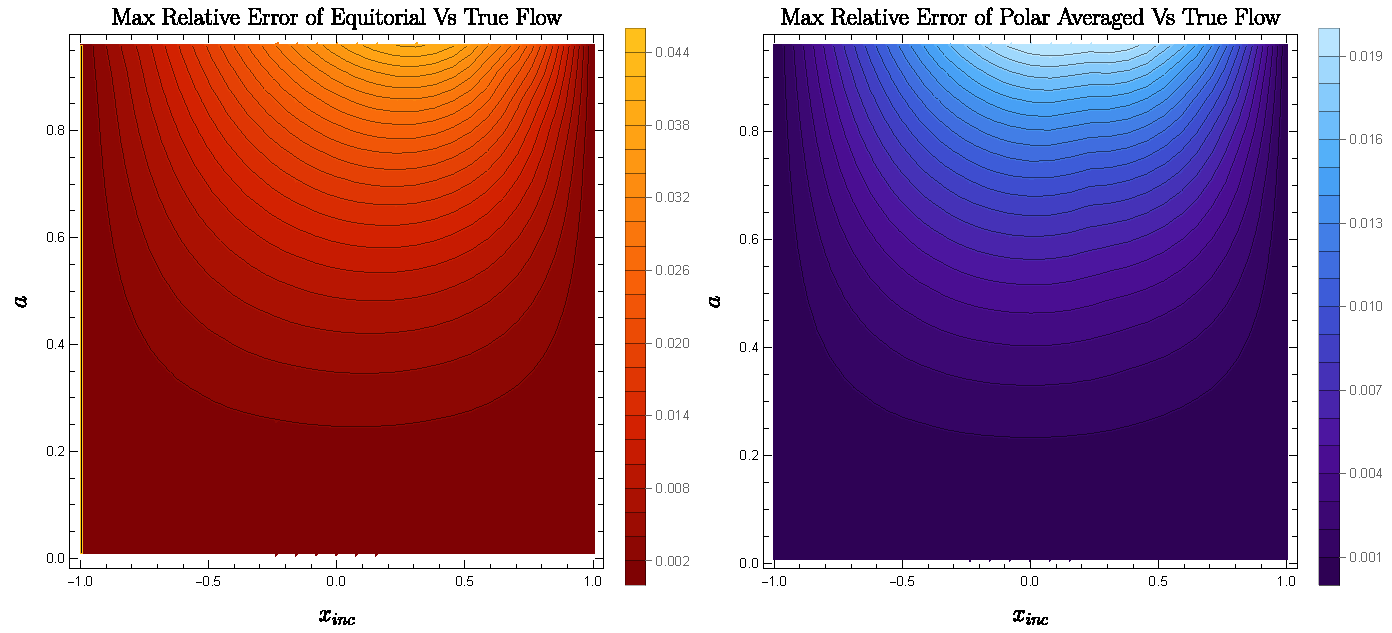
\includegraphics[width=150mm]{ContourFLows.pdf}
        \caption{Left Image: Plot of the maximum relative error between the equatorial and true flow over the range $(r_+,r_I)$. Right Image: Plot of the maximum relative error between the polar averaged and true flow over the range $(r_+,r_I)$.}
    \label{fig:flowerrors}
\end{figure}


\subsection{Solutions to the equations of motion}
At this stage we are now ready to solve the equations of motion. In the generic case we expect the solutions to arise in terms of elliptic functions. In the ISSO case however we find that the triple root in fact simplifies the terms with radial dependence to the form of elementary functions. For convenience the solutions for the entirety of the ISSO case are given with initial conditions $(t(\lam),r(\lam),z(\lam),\phi(\lam))|_{\lam=0} =(0,r_4,0,0)$. The full solution can be easily reconstructed using Eq.~\eqref{eq:MINOISSO}.
\subsubsection{Radial Equation}
Solving Eq.~\eqref{eq:ISSOradialeom} and inverting the solution gives 
    \begin{align}\label{eq:MINOISSO}
        \lambda(r) = \frac{2\sqrt{r-r_4}}{\sqrt{(1-\EN^2)(r_I-r)(r_I-r_4)^2}},
    \end{align}
and
\begin{align}
        r(\lambda) = \frac{r_I(r_I-r_4)^2(1-\EN^2)\lambda^2+4r_4}{(r_I-r_4)^2(1-\EN^2)\lambda^2+4}
\end{align}
respectively.
\subsubsection{Polar Equation}
We then find the solution for the polar equation to be given by 
\begin{equation}\label{Eq:ISSOPolar}
    z(\lambda) = z_1 \sin{\xi_z(\lam)}.
\end{equation}
Here we have defined,
\begin{equation}
    \xi_z(\lam)= \am(z_2 \lam| k_z^2),
\end{equation}
where $\am(\cdot|\cdot)$ is the standard Jacobi amplitude function. 
Conveniently for the remaining equations of motion the polar and radial dependence in the time and azimuthal equation fully decouple from each other in Mino time. This means we are only required to resolve the radial component as the polar part will simply remain the same as has already been found for bound orbits in~\cite{Fujita:2009bp,vandeMeent:2019cam}. The polar dependence still remains in the form of elliptic integrals whereby $\elF(\cdot)$, $\elE(\cdot)$ and $\mathrm{\Pi}(\cdot)$ are the elliptic integral of the first, second and third kind respectively.
\subsubsection{Azimuthal Equation}

Going on to solve the azimuthal component we first rewrite Eq.~\eqref{eq:azimuthaleom} as
\begin{align}
\begin{aligned}
        d\phi &= \frac{-a}{\Delta}\frac{\mathcal{E}(r^2+a^2)-a\mathcal{L}}{\sqrt{(1-\EN^2)(r_I-r)^3(r-r_4)}}dr\\
        &\qquad+\frac{\mathcal{L}}{1-z^2}\frac{1}{\sqrt{(z^2-z_1^2)(a^2(1-\EN^2) z^2-z_2^2)}}dz
        -a\mathcal{E}d\lam. 
\end{aligned}
\end{align}
We then integrate each of the terms individually. The component comprising of r dependence is found to be given by,
\begin{align}
\begin{aligned}
    \phi_r(\lam)& = a \frac{(\EN(r_I^2+ a^2) - a \ANG)\lam }{(r_I-r_{-})(r_I-r_{+})} \\
    &+ \frac{a}{\sqrt{(1-\EN^2)}}\bigg(\frac{(\EN(r_{-}^2+ a^2) - a\ANG)
   \ln\left({\sqrt{\frac{\big(2\sqrt{r_{-}-r_4}+\lam(r_I-r_4)\sqrt{(1-\EN^2)(r_I-r_-)}\big)^2}{\big(2\sqrt{r_{-}-r_4}-\lam(r_I-r_4)\sqrt{(1-\EN^2)(r_I-r_-)}\big)^2}}}\right)}{\sqrt{r_{-}-r_4}(r_I-r_{-})^{\frac{3}{2}}(r_{+}-r_{-})}\\
   &\;\;\;\;\;\;\;\;\;\;\;\;\;\;\;\;\;\;\;\;\;\;\;\;\;\;\;\;\;\;\;\;\;\;\;\;\;\;\;\;\;\;\;\;\;\;\;\;\;\;\;\;\;\;\;\;\;\;\;\;\;\;\;\;\;\;\;\;\;\;\;\;\;\;\;\;\;\;\;\;\;\;\;\;\;+ (r_{-} \Longleftrightarrow r_{+}) \bigg).
\end{aligned}
\end{align}
Where the arrow notation denotes taking the other term within the shared brackets and swapping all occurrences of $r_-$ with $r_+$ and vice-versa. The component with $z$ dependence is then given by,
\begin{align}
    \phi_z(\lam) = \frac{\ANG}{z_2}  \elPi(z_1^2; \xi_z(\lam) | k_z^2 ).
\end{align}
The polar average form of this solution can also be found dramatically simplifying the functional dependence and is given by,
\begin{align}
    \langle \phi_z \rangle_z(\lam) = \frac{\ANG}{ \elK(k_z^2)}\elPi(z_1^2; k_z^2 ) \lam.
\end{align}
Where $\elPi(\cdot,\cdot)$ is the complete elliptic integral of the third kind. Thus we find the full azimuthal solution to be given by 
\begin{align}
    \phi(\lam) = \phi_r(\lam) + \phi_z(\lam) - a \EN \lam.
\end{align}
\subsection{Time Equation}
We perform a similar separation in the integration of the equation of motion for coordinate time giving,

\begin{align}
\begin{aligned}
    t_r(\lam) &= \frac{(a^2+r_I^2)(\EN(r_I^2+ a^2) - a \ANG)\lam }{(r_I-r_{-})(r_I-r_{+})}+ \frac{2(r_I - r_4)^2\EN \lam}{4 + (1-\EN^2)(r_I-r_4)^2\lam^2}\\
    &- \frac{(r_4+3r_I + 2(r_{+}+r_{-}))}{\sqrt{(1-\EN^2)}}\EN\arctan \left( \frac{\lam (r_I-r_4)\sqrt{(1-\EN^2)}}{2}\right)\\
    &+ \Biggl( \frac{(a^2+r_{-}^2)(\EN(r_{-}^2+ a^2) - a \ANG)  \ln\bigg({\sqrt{\frac{\big(2\sqrt{r_{-}-r_4}+\lam(r_I-r_4)\sqrt{(1-\EN^2)(r_I-r_-)}\big)^2}{\big(2\sqrt{r_{-}-r_4}-\lam(r_I-r_4)\sqrt{(1-\EN^2)(r_I-r_-)}\big)^2}}}\bigg)}{\sqrt{r_{-}-r_4}(r_I-r_{-})^{\frac{3}{2}}(r_{+}-r_{-})\sqrt{(1-\EN^2)}} \\
    &\;\;\;\;\;\;\;\;\;\;\;\;\;\;\;\;\;\;\;\;\;\;\;\;\;\;\;\;\;\;\;\;\;\;\;\;\;\;\;\;\;\;\;\;\;\;\;\;\;\;\;\;\;\;\;\;\;\;\;\;\;\;\;\;\;\;\;\;\;\;\;\;\;\;\;\;\;\;\;\;\;\;\;\;\;+ (r_{-} \Longleftrightarrow r_{+}) \Biggl).
\end{aligned}
\end{align}
We next find the polar dependant part of the time solution to be given by,
\begin{align}
    \begin{aligned}
    t_z(\lam)  = \frac{ \EN}{1-\EN^2}\left( (z_2^2 - a^2(1-\EN^2))\lam - z_2\elE(\xi_z(\lam)|k_z^2) \right),
    \end{aligned}
\end{align}
and the polar averaged form of this solution is given by, 
\begin{align}
    \begin{aligned}
   \langle t_z\rangle_z (\lam)  = \frac{z_2^2 \EN}{1-\EN^2}\left( 1 - \frac{a^2(1-\EN^2)}{z_2^2} - \frac{\elE( k_z^2)}{ \elK(k_z^2)} \right)\lam.
    \end{aligned}
\end{align}
This is the expression we required to derive the polar averaged radial flow in Eq.~\eqref{eq:radialinflowPolarAVG}.
Putting this all together we then find the full time solution to be given by 
\begin{align}
    t(\lam) = t_r(\lam) +   t_z(\lam) + a \ANG \lam.
\end{align}
We find that all of the novel radial integrals which are required to be solved can be done so without too much issue through the use of partial fractions. They can then be fully analytically continued by applying some simple trigonometric substitutions.

\begin{figure}[tb!]
\centering
    \includegraphics[width=100mm]{ISSOPlots.pdf}
    \caption{Orbital plots of plunging geodesics which asymptote to the ISSO in the infinite past $(a,r_I) = (0.9,2.6)$ and $\theta = \mathrm{arccos}(z)$. Here the cyan and orange planes are the azimuthally co-precessing and poloidally co-rotating planes respectively. } 
    \label{fig:ISSOplots}
\end{figure}
From Fig.~\ref{fig:ISSOplots} it can now be explicitly seen that enforcing the triple root places us in a regime where in the infinite past a test particle on these geodesic has asymptoted from the ISSO to subsequently plunge in through the horizon. These showcase a number of properties of the plunge in Boyler-Lindquist co-ordinates. The structure of these geodesics is more easily depicted when orthogonally projected onto a azimuthally co-precessing and poloidally co-rotating plane fixed to a particle as it follows the geodesic  Fig.~\ref{fig:coorotatingISSOplots}.
\begin{figure}[tb!]
    \centering
    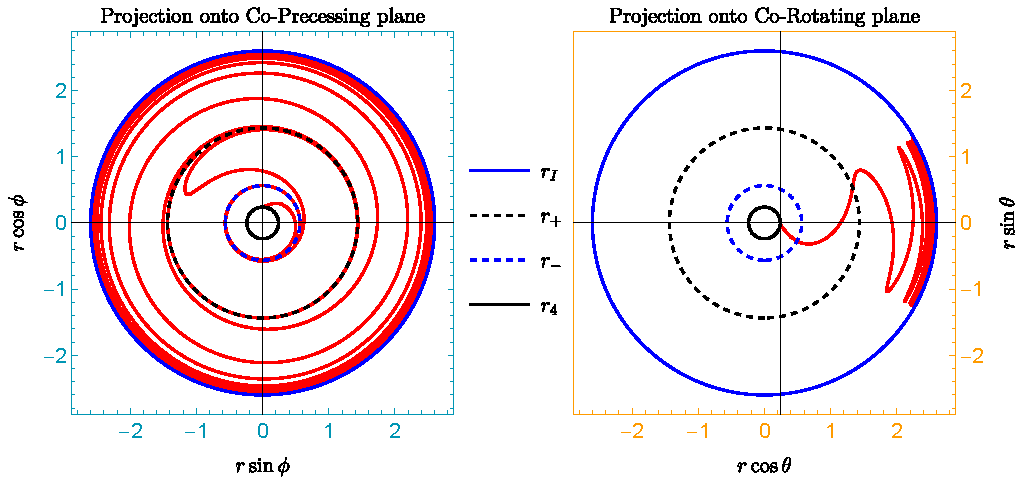
\includegraphics[width=140mm]{corotatingISSOPlots.pdf}
    \caption{Co-rotating orbital plots of plunging geodesics which asymptote to the ISSO in the infinite past $(a,r_I) = (0.9,2.6)$ . Left Image: orthogonal projection of ISSO plunge onto the co-precessing azimuthal plane. Right Image: orthogonal projection of ISSO plunge onto co-rotating polar plane.}
    \label{fig:coorotatingISSOplots}
\end{figure}

In Fig.~\ref{fig:coorotatingISSOplots} we see that the azimuthal coordinate diverges at both the inner and outer horizons. Analysis of the coordinate time solution shows it also diverges at these points, this occurs for a similar reason as to the coordinate time diverges at the horizon in Schwarzchild coordinates for a non-spinning black hole, due to the infinite redshift. In much the same way as we have an infinite redshift on the hoirzon one can intuitively think of this azimuthal divergence occurring as a consequence of the infinite redshift on the horizon forcing the geodesics to also corotate with the black hole an infinite number of times before passing through the horizon. Naturally this is only a co-ordinate singularity and the process occurs in finite Mino and proper time. Due to this discontinuity car must be taken in the choice of branch between $r_+$ and $r_-$, as the direction of motion between the horizons seems to invert but it can be checked that our solutions conserve $\EN,\ANG$ and $Q$ throughout their parameterisation. In addition the issue of reaching a manifold singularity can only occur when the geodesics is confined to the equatorial plane  \cite{Hackmann:2010zz}. Finally we note if one measures both the spin $(a)$ and $r_{ISSO}$ of an astrophysical black hole then one can immediately determine $(\EN,\ANG,Q)$ allowing them to calculate $z_1(a,r_{ISSO})$. As $z_1$ directly corresponds to the amplitude of the oscillation at $r_I$, being able to determine this quantity analytically provides a direct means of bounding the thickness at the order of geodesic motion of an accretion disk at $r_{ISSO}$.

\section{Generic plunge orbits}\label{sec:deeplybound}
For the case of generic plunge orbits the integrals we are required to compute are notably more involved. In the case with $R(r)$ having four real roots ($r_4<r_3<r_2<r_1$) with  $r_4<r_-<r_+<r_3<r_2<r_1$  the solution can be directly borrowed from the bound orbit case \cite{vandeMeent:2019cam,Fujita:2009bp}  with the modification of $r_1 \Longleftrightarrow r_3$ and  $r_2 \Longleftrightarrow r_4$. In addition in the case of 4 real roots  ($r_4<r_3<r_2<r_1$) with $r_4<r_3<r_2<r_-<r_+<r_1$ then the solutions can again be found from \cite{vandeMeent:2019cam,Fujita:2009bp} this time with no modification. In the case of two real and two complex roots however, we are required to begin the procedure of solving the complicated elliptic integrals from scratch if we wish to find an analytic form that is manifestly real.


\subsection{Generic plunge orbits with two complex roots}
In calculating the integrals for this case we follow the procedure outlined in \cite{LabanMutrie} and give an overview of the steps involved. We begin by again noting  that only the radial components of each of the equations need to be solved as the other remaining terms are identical to those already found in the ISSO case above. Recall we now have the general expression $R(r) = (\mathcal{E}(r^2+a^2)-a\mathcal{L})^2-\Delta(r^2+(a\mathcal{E}-\mathcal{L})^2+Q)$ where $\EN$, $\ANG$ and $Q$ are all now independent quantities. At this stage the integrals of concern are given by 
\begin{align}\label{Kerr EOM}
    \begin{aligned}
        \lambda &= -\int\frac{dr'}{\sqrt{ R(r')}},\\
        t_r(r) &= -\int \frac{(r'^2+a^2)(\EN(r'^2+a^2)-a\mathcal{L}) dr'}{\Delta\sqrt{ R(r')}}\;\; \text{and} \\
        \phi_r(r) &= -\int \frac{a(\mathcal{E}(r'^2+a^2)-a\mathcal{L})dr'}{\Delta\sqrt{ R(r')}}. 
    \end{aligned}
\end{align}
Note that although these integrals look to be of the same form as those we just solved for the ISSO case without much mention, the reason for the substantial increase in complexity is due to the fact that $R(r)$, in general, no longer contains any double or triple roots forcing us to much more carefully consider the elliptic integrals at hand. The key idea in the procedure we wish to apply is that at the end we should only have integrals of the form
\begin{align}\label{eq:ellipticBasis}
    \begin{aligned}
     &\lam = -\int\frac{dr}{\sqrt{ R(r)}},\;\;\; \mathcal{I}_r = \int\frac{rdr}{\sqrt{ R(r)}},\\
     &\mathcal{I}_{r^2} = \int\frac{r^2dr}{\sqrt{ R(r)}}\;\; \text{and} \;\;\mathcal{I}_{r_{\pm}} = \int\frac{dr}{(r-r_{\pm})\sqrt{ R(r)}}
    \end{aligned}
\end{align}
appearing in our equations. We solve these integrals in terms of the radial co-ordinate $r$ which we can later parameterise by $\lam$ by inverting the solution of $\lam = -\int^{r}\frac{dr'}{\sqrt{ R(r')}}$.

We begin solving the equations by continually applying partial fractions to the radial part of the $\phi$ and $t$ equations until arriving at the form
\begin{equation}\label{eq:reducedformphi }
        \phi_r = a\left( \frac{(\EN(r_-^2+ a^2) - a \ANG)}{(r_{-}-r_{+})} \mathcal{I}_{r_{-}} + (r_{-} \Longleftrightarrow r_{+})\right) + a \EN \lam,
\end{equation}
and
\begin{align}\label{eq:reducedformt}
\begin{aligned}
    t_{r} = \EN(r_{+}^2&+r_{-}^2 + r_{+}r_{-}+2a^2)\lam + \EN\left(\mathcal{I}_{r^2} +  \mathcal{I}_{r}(r_{-} +r_{+})\right)\\
    &+\left(\frac{(r_{-}^2+a^2)(\EN(r_-^2+ a^2) - a \ANG)}{r_{-}-r_{+}}\mathcal{I}_{r_{-}} + (r_{-} \Longleftrightarrow r_{+})\right)-a \ANG \lam.
\end{aligned}
\end{align}
At this point we can now concentrate on calculating the four elliptic integrals defined in Eq.\eqref{eq:ellipticBasis}. We do this my applying a transformation given for the case of two complex roots in \cite{LabanMutrie}. This procedure begins by letting $R(r)$ have two real roots $r_1 < r_2$ and two complex roots $r_3$ and $r_4$. We then rewrite $R(r)$ in the form $R(r) = (1-\EN^2)(r_2-r)(r-r_1)(r^2 - 2\rho_rr + \rho_r^2 -\rho_i^2) $ where  $\rho_r=\Re(r_3)$ and $\rho_i=\Im(r_4)$. Further we define
\begin{align}
    \begin{aligned}
A &= \sqrt{(r_2-\rho_r)^2+\rho_i^2} , \;\;\;B = \sqrt{(r_1-\rho_r)^2+\rho_i^2} ,\\ 
f &= \frac{4 A B}{(A-B)^2},\;\;\;k_r = \sqrt{\frac{(r_2-r_1)^2 - (A-B)^2}{4 A B }}, \;\;\; \\
p_2 &= r_1A^2+r_2B^2-(r_2+r_1)AB
    \end{aligned}
\end{align}
and 
\begin{align}
        \xi_r(\lam) &= \am(\sqrt{ (1-\EN^2) A B} \lam|k_r^2).\label{eq:xiR}
\end{align}
 Next motivated by the tables provided in \cite{LabanMutrie} we make the substitution in the integrals Eq.~\eqref{eq:ellipticBasis} of the form, 
\begin{equation}\label{eq:transformation}
    r(y) = \frac{p_2y^2+2(r_2+r_1)AB+2(r_2-r_1)AB\sqrt{1-y^2}}{(A-B)^2y^2+4AB}.
\end{equation}
Applying this transformation to Eq.~\eqref{eq:ellipticBasis} and again repeatedly applying partial fractions we find each integral reduces to sum over elliptic integrands and rational polynomials. Integrating over the latter terms will always provide elementary functions and integrals over the former will of course give elliptic functions. The solutions we then obtain are only analytic on the range $r\in (r_1, \frac{r_2A+r_1B}{A+B})$ where for convenience we have set the initial conditions to be given by $(t(\lam),r(\lam),z(\lam),\phi(\lam))|_{\lam=0} =(0,r_1,0,0, )$. Next we analytically extend these solutions through the point $r =\frac{r_2A+r_1B}{A+B}$ by use of trigonometric and elliptic substitutions providing a fully analytic solution on the range $r\in(r_1,r_2)$. The fully analytical solution to these integrals is then given by
\begin{equation}\label{eq:MINOsolution}
     \int\frac{dr}{\sqrt{ R(r)}} = \frac{1}{\sqrt{(1-\EN^2)A B}} \elF\left( \frac{\pi}{2}-
\arcsin\left(\frac{B(r_2-r) - A(r-r_1)}{ B(r_2-r)+A(r-r_1)}\right)\bigg| k_r^2\right),
\end{equation}

\begin{equation}\label{eq:Ir}
    \begin{aligned}
   \mathcal{I}_r(\lam) =\frac{Ar_1-Br_2}{A-B}\lam -\frac{1}{\sqrt{(1-\EN^2)}}&\arctan  \left( \frac{(r_2-r_1)}{2\sqrt{AB}}\frac{\snr}{\sqrt{1-k_r^2\snr^2}}\right)\\
    & + \frac{(A+B)(r_2-r_1)}{2(A-B)\sqrt{(1-\EN^2) A B}}\elPi\left( -\frac{1}{f}; \amr|k_r^2\right),
    \end{aligned}
\end{equation}
\begin{equation}\label{eq:Ir2}
    \begin{aligned}
   \mathcal{I}_{r^2}&(\lam) =\frac{(Ar_1^2-Br_2^2)}{(A-B)}\lam + \frac{\sqrt{AB}}{(1-\EN^2)}\elE\left(\amr|k_r^2\right)\\
  &- \frac{(A+B)(A^2+2r_1^2-B^2-2r_2^2)}{4(A-B)\sqrt{(1-\EN^2) A B}}\elPi(-\frac{1}{f};\amr|k_r^2)\\
  &-\frac{\sqrt{A B}(A+B-(A-B)\cnr)}{(A-B)\sqrt{(1-\EN^2)}}\frac{\snr\sqrt{1-k_r^2\snr^2}}{(f+\snr^2)}\\
  &+\frac{A^2+2r_1^2-B^2-2r_2^2}{4(r_2-r_1)\sqrt{(1-\EN^2)}}\times\\
  \;\;\;\;\;\;\;&\arctan\left(f - (1+2 f k_r^2)\sin^2(\xi_r), 2 \sin(\xi_r) \sqrt{1-k_r^2\sin^2(\xi_r)}\sqrt{f(1+f k_r^2)}\right) 
    \end{aligned}
\end{equation}  
and
\begin{equation}\label{eq:Irpm}
    \begin{aligned}
   \mathcal{I}_{r_{\pm}}(\lam) &= \frac{(A-B)\lam}{A(r_1-r_{\pm})-B(r_2-r_{\pm})} \\
   &+ \frac{(r_2-r_1)(A(r_1-r_{\pm})+B(r_2-r_{\pm}))}{2\sqrt{(1-\EN^2) A B}(r_{\pm}-r_1)(r_2-r_{\pm})(A(r_1-r_{\pm})-B(r_2-r_{\pm}))}\elPi\left(\frac{1}{D_{\pm}^2}; \amr|k_r^2\right)\\
   -&\frac{\sqrt{r_2-r_1} \ln\left( \frac{\big(D_{\pm} \sqrt{1-D_{\pm}^2k_r^2} + \sqrt{1-k_r^2\snr^2}\snr\big)^2+ \big(k_r(D_{\pm}^2-\snr^2)\big)^2}{\big(D_{\pm} \sqrt{1-D_{\pm}^2k_r^2} -\sqrt{1-k_r^2\snr^2}\snr\big)^2+ \big(k_r(D_{\pm}^2-\snr^2)\big)^2}\right)
    }{4\sqrt{(1-\EN^2)(r_2-r_{\pm})(r_{\pm}-r_1)}\sqrt{(A^2(r_{\pm}-r_1)-(r_2-r_{\pm})(r_1^2-B^2+r_2r_{\pm}-r_1(r_2+r_{\pm}))}}
    \end{aligned}
\end{equation}
with,
\begin{align*}
    D_{\pm} = \frac{\sqrt{4AB(r_2-r_{\pm})(r_{\pm}- r_1)}}{A(r_{\pm}-r_1)+B(r_{\pm}-r_2)}
\end{align*}
Where we note that $\xi_r$ has explicit dependence on $\lam$ as seen in Eq.~\eqref{eq:xiR}, we have not explicitly stated it in the above in the interest of readability. The $\arctan$ function seen in Eq.~\eqref{eq:Ir2} is the two argument arctan function which tracks the sectors of the numerator and denominator.
\subsection{Solutions to Equations of Motion}
At this point the solution for Eqs.~\eqref{eq:MINOsolution}-\eqref{eq:Irpm} for the elliptic integrals can then be readily substituted back into Eq.~\eqref{eq:reducedformphi } and  Eq.~\eqref{eq:reducedformt} giving the full form of the solutions to generic plunges. Also note that all z dependant quantities such as $z, \phi_z$ and $t_z$ do not need to be solved again as they will be equivalent to the ISSO case. We present all solutions parameterised in terms on mino time $(\lam)$ which is done by simply inverting the solution to Eq.~\eqref{eq:MINOsolution} to obtain $r(\lam)$ then substituting the solution for $r(\lam)$ everywhere $r$ appears in  Eqs.~\eqref{eq:Ir}-\eqref{eq:Irpm} . Following this substitution the equations then require some further massaging but can be given in a form fully analytic on $\lam \in (-\infty,\infty)$ with the exception of a countable number of singularities corresponding to repeated crossings of horizons which we expect in Boyer-Lindquist coordinates. With this we can now readily attain the solution to the generic timelike plunging geodesics.


The radial equation is first found by simply inverting the solution for Eq.~\eqref{eq:MINOsolution} to give,
\begin{equation}
r(\lam) = \frac{(A-B)(Ar_1-Br_2)\snr^2+2A B(r_1+r_2)-2AB(r_2-r_1)\cnr}{4 A B + (A-B)^2 \snr^2}.
\end{equation}
The solutions to the polar equation remain the same as for the ISSO case. 
    
Taking Eq.~\eqref{eq:reducedformphi } the solution  to the azimuthal equations of motion can then immediately be found from the solutions of Eq.~\eqref{eq:ellipticBasis}

\begin{align}
    \phi(\lam) = \phi_r(\lam) + \phi_z(\lam) - a \EN \lam
\end{align}   
similarly to the azimuthal case from Eq.~\eqref{eq:reducedformt} we can now immediately obtain
\begin{align}
    t(\lam) = t_r(\lam) +   t_z(\lam) +a \ANG \lam,
\end{align}
where both $\phi_z$ and $t_z$ can be immediately be taken from the ISSO case. Having attained the full set of solutions for generic plunges one can plot the spatial component depicting the orbital evolution of the generic plunging geodesics Fig.~\ref{fig:genericplots}. 
\begin{figure}[tb!]
    \centering
    \includegraphics[width=100mm]{GenericPlots.pdf}
         \caption{Orbital plots of generic plunging geodesics with parameter values $(a,\EN,\ANG,Q) = (0.9,0.94,0.1,12)$ and $\theta = \mathrm{arccos}(z)$. The larger black sphere gives the horizon of the black hole where as the smaller sphere simply gives a point along the geodesics. Here the cyan and orange planes are the azimuthally co-precessing and poloidally co-rotating planes respectively. }
    \label{fig:genericplots}
\end{figure}
\begin{figure}[tb!]
    \centering
    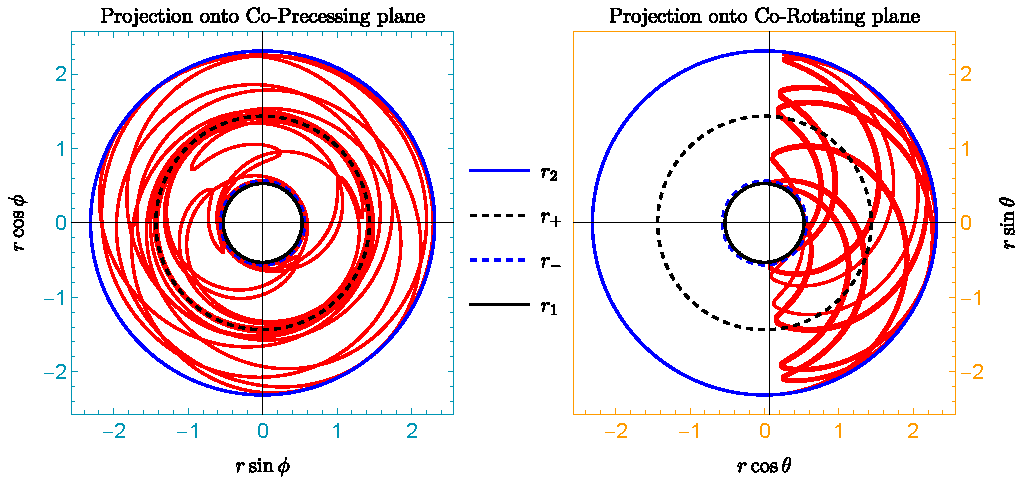
\includegraphics[width=150mm]{corotatingGenericPlots.pdf}
    \caption{Corotating orbital plots of generic plunging geodesics with parameter values $(a,\EN,\ANG,Q) = (0.9,0.94,0.1,12)$. Left Image: orhtogonal projection of generic plunge onto the co-precessing azimuthal plane. Right Image: orthogonal projection of generic plunge onto co-rotating polar plane.}
    \label{fig:coorotatinggeneric}
\end{figure}
More informatively the orthogonal projection onto the azimuthaly co-precessing and poloidaly co-rotating planes in Fig.~\ref{fig:coorotatinggeneric} again show the divergences at either horizon in the $\phi$ coordinate. Importantly, once we have constructed these solution we check that $\EN$ and $\ANG$ are indeed still conserved by evaluating $ -u^{\nu}g_{\mu\nu}\left(\frac{\partial}{\partial t}\right)^{\nu}$ and $ u^{\nu}g_{\mu\nu}\left(\frac{\partial}{\partial \phi}\right)^{\nu} $ explicitly. We find this is the case for all values of $\lam$ not only acting as a consistency check of our equations but also showing we have selected the correct branches of the solution between each of the horizon divergences. We then substitute our solutions back in the equations of motion for both the ISSO and generic case and find that everything remains consistent. Finally from out solutions the radial and polar frequencies for a generic plunge can be obtained and are given by
\begin{align}
    \Upsilon_r &=  \frac{\sqrt{ A B(1-\EN^2)}}{2 \elK(k_r^2)}, \\
    \Upsilon_z &= \frac{\pi \elK(k_z^2)}{2 z_2}.
\end{align}

\section{Discussion}\label{sec:conclusion}
\mvdm{In this work we have given the full closed form analytic solution for \cd{generic} bound plunges into a Kerr black hole. We have paid particular attention to the special edge case of plunges starting asymptotically from the innermost stable precessing circular orbit (ISSO), in which the solutions take a particularly simple form, generalizing the result of~\cite{Mummery:2022ana}. The general expression for the inflow in this case, is more involved due to oscillations coming from the polar motion. We have therefore provide two simplified approximations for the inflow rate, and assess their accuracy.

The geodesics asymptoting from the ISSO can be parameterized purely in terms of black hole spin and the radius of the ISSO. In the equatorial case, the black hole spin determines one prograde and one retrograde ISCO. In the inclined case the black hole spin now defines a range of allowed radii for the ISSO each of which corresponding to a unique inclination in either prograde or retrograde. We expect these solutions to be relevant in the case of accretion disk astrophysics where our equations should have considerable applications in the analytic modelling of accretion disk flow into the black hole.
}

The provided explicit solutions for plunging geodesics are expected to find practical use in modelling the inspiral of binary black holes, since in the small mass-ratio limit they will describe the final phase of the inspiral before merger. As small mass-ratio methods are applied to more equal mass systems, including this phase becomes increasingly important. For ease of application we have incorporated our results in the {\tt KerrGeodesics} package in the Black hole perturbation toolkit \cite{BHPToolkit}.

In this work we have restricted attention to ``bound'' plunge geodesics, i.e. geodesics with $\EN<1$. In principle, the explicit solutions given here can easily be extended to the case of ``direct plunges'' coming from infinity and falling into the black hole, or deeply bound plunges inside a scattering geodesic. In both cases, this involves taking the expressions in this paper in terms of the outermost real root and analytically continuing it past positive infinity to negative value (e.g. by considering the reciprocal root). However, this will not necessarily give all  $\EN>1$ plunging geodesics, which also includes so-called ``vortical'' geodesics with negative values of $Q$.

We have also considered only the special edge case of plunges asymptoting from the ISSO. In general, the

\cd{ In preparation of this manuscript, \cite{Mummery:2023hlo} submitted work which is distinct from, but relevant to the work we have presented in this paper.}

\section*{Acknowledgements}
We acknowledge support from the Villum Investigator program supported by the VILLUM Foundation (grant no. VIL37766) and the DNRF Chair program (grant no. DNRF162) by the Danish National Research Foundation. This work makes use of the Black Hole Perturbation Toolkit \cite{BHPToolkit}.
\section*{References}
\bibliography{references}


\appendix
\section{Range of allowed $r_I$ for a given spin for ISSO plunges}\label{app:ISSOrange}

Defining $\chi =(27-45a^2+17a^4+a^6+8 a^3(1-a^2))^{\frac{1}{3}} $ and $\psi = \sqrt{3 + a^2 + \frac{9-10a^2+a^4}{\chi} +\chi} $ the range of possible $r_{I}$ values for a given $a$ are,
\begin{align}\label{eq:RIminmax}
    R_{I,\rm min/max} = 3 + &\psi \mp \frac{1}{2}\sqrt{\left( 72+8(a^2-6)-\frac{4(9-10a^2+a^4)}{\chi}-4\chi+\frac{64a^2}{\psi} \right).}
\end{align}

\section{Value of $\ANG_{\rm root}$ for ISSO Plunges parameterised by $r_I$}\label{app:Lroot}
Defining $\kappa = \sqrt{a^2-2r+r^2}$ the value of $\ANG_{\rm root}$ is given as the root of the function 
\begin{align}
\begin{aligned}\label{eq:Lroot}
        \alpha(r) = a^6 - 3 a^2 r^{\frac{5}{2}}( 3 r^{\frac{3}{2}}+  &\kappa( 6 - 2r))+r^{\frac{9}{2}}(r^{\frac{1}{2}}(20 -11r) + \kappa(5 + 3r))\\
        &+ a^4( r(3r -4) + \kappa r^{\frac{1}{2}}(1 + 3r) ),  
\end{aligned}
\end{align}
which is real and closest to $r = 6$. Eq.~\eqref{eq:Lroot} has been given in a form such that the root can be found numerically to high precision which is not the case for Eq.~\eqref{eq:ANG}.

\section{Proper time solution for ISSO plunges}\label{app:ISSOproper}

To connect back to a more physical intuition we also provide a solution for the proper time in terms of Mino time for the case of ISSO plunges.
\begin{align}
    \tau_r(\lam) =&\left(r_I^2+\frac{2(r_I-r_4)^2}{4 + (1-\EN^2)(r_I-r_4)^2\lam^2}\right)\lam+ \frac{ (r_4^2 +2r_4r_I-3r_I^2)\arctan(\frac{\lam(r_I-r_4)\sqrt{(1-\EN^2)}}{2})}{\sqrt{(1-\EN^2)}(r_I-r_4)}
\end{align}
\begin{align}
    \tau_z(\lam) =&\frac{ z_2 }{(1-\EN^2)}\left( F(\amz|k_z^2 )-E(\amz|k_z^2)\right)
\end{align}
\begin{align}
    \tau(\lam) =& \tau_r(\lam)+ \tau_z(\lam)
\end{align}


\section{Proper time solution time for generic plunges with 2 complex roots}\label{app:2Cproper}
\begin{align}
    \tau_r(\lam) =\mathcal{I}_{r^2}(\lam) 
\end{align}
\begin{align}
    \tau_z(\lam) =&\frac{ z_2 }{(1-\EN^2)}\left( F(\amz|k_z^2 )-E(\amz|k_z^2)\right)
\end{align}
\begin{align}
    \tau(\lam) =& \tau_r(\lam)+ \tau_z(\lam)
\end{align}

\end{document}

